% !TEX TS-program = lualatex
\documentclass[tikz,border=6pt]{standalone}

\usepackage{amsmath,amssymb}
\usetikzlibrary{arrows.meta,calc,decorations.markings,positioning}

\begin{document}
	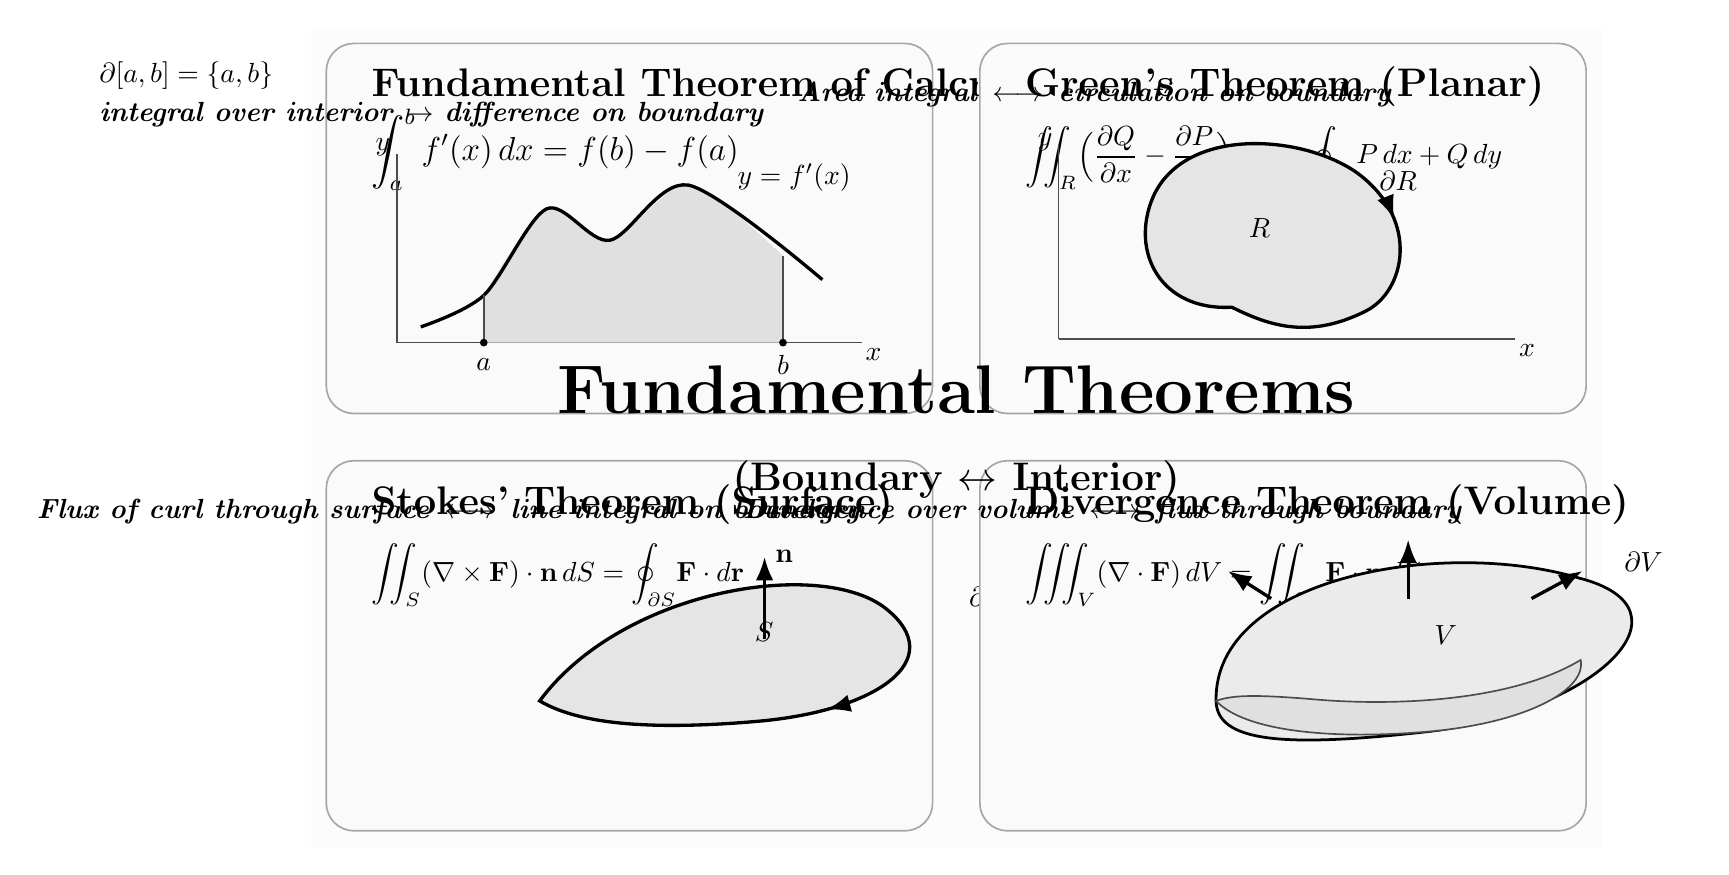
\begin{tikzpicture}[
		font=\sffamily,
		>=Latex,
		panel/.style={rounded corners=10pt, line width=0.6pt, draw=black!35, fill=black!2},
		title/.style={font=\bfseries\Large, align=left},
		formula/.style={font=\bfseries\large, align=left},
		smallformula/.style={font=\bfseries\normalsize, align=left},
		axis/.style={line width=0.6pt, draw=black!70},
		curve/.style={line width=1.2pt, draw=black},
		boundary/.style={line width=1.2pt, draw=black, -{Latex[length=3mm]}},
		boundaryloop/.style={
			line width=1.2pt, draw=black,
			postaction={decorate},
			decoration={markings, mark=at position 0.65 with {\arrow{Latex[length=3mm]}}}
		}
		]
		
		% --- overall background (optional) ---
		\fill[black!1] (-0.2,-0.2) rectangle (16.2,10.2);
		
		% layout parameters
		\def\W{7.7} % panel width
		\def\H{4.7} % panel height
		\def\gap{0.6}
		
		% panel origins
		\coordinate (P1) at (0,5.3);
		\coordinate (P2) at (\W+\gap,5.3);
		\coordinate (P3) at (0,0);
		\coordinate (P4) at (\W+\gap,0);
		
		% =========================================================
		% Panel 1: 1D FTC
		% =========================================================
		\begin{scope}[shift={(P1)}]
			\path[panel] (0,0) rectangle (\W,\H);
			
			\node[title, anchor=west] at (0.45,\H-0.55) {Fundamental Theorem of Calculus (1D)};
			\node[formula, anchor=west] at (0.45,\H-1.35)
			{$\displaystyle \int_a^b f'(x)\,dx = f(b)-f(a)$};
			
			\draw[axis] (0.9,0.9) -- (0.9,3.3);
			\draw[axis] (0.9,0.9) -- (6.8,0.9);
			\node[font=\normalsize] at (6.95,0.75) {$x$};
			\node[font=\normalsize] at (0.72,3.38) {$y$};
			
			% Fill Area
			\coordinate (a) at (2.0,0.9);
			\coordinate (b) at (5.8,0.9);
			
			\path[fill=black!12]
			(a) -- plot[smooth] coordinates {(2.0,1.5) (2.8,2.6) (3.6,2.2) (4.6,2.9) (5.8,2.0)}
			-- (b) -- cycle;
			
			% Draw Curve
			\draw[curve]
			plot[smooth] coordinates {(1.2,1.1) (2.0,1.5) (2.8,2.6) (3.6,2.2) (4.6,2.9) (6.3,1.7)};
			\node[font=\normalsize, anchor=west] at (5.1,3.0) {$y=f'(x)$};
			
			% Boundary Lines
			\draw[axis] (a) -- (2.0,1.5);
			\draw[axis] (b) -- (5.8,2.0);
			\node[font=\normalsize] at (2.0,0.62) {$a$};
			\node[font=\normalsize] at (5.8,0.62) {$b$};
			
			\fill[black] (a) circle (1.4pt);
			\fill[black] (b) circle (1.4pt);
			
			\node[font=\bfseries\normalsize, align=left] at (1.35,4.05)
			{$\partial[a,b]=\{a,b\}$\\[2pt] \textit{integral over interior} $\rightarrow$ \textit{difference on boundary}};
		\end{scope}
		
		% =========================================================
		% Panel 2: Green's Theorem
		% =========================================================
		\begin{scope}[shift={(P2)}]
			\path[panel] (0,0) rectangle (\W,\H);
			
			\node[title, anchor=west] at (0.45,\H-0.55) {Green's Theorem (Planar)};
			\node[smallformula, anchor=west] at (0.45,\H-1.45)
			{$\displaystyle \iint_{R}\!\Big(\frac{\partial Q}{\partial x}-\frac{\partial P}{\partial y}\Big)\,dA
				= \oint_{\partial R}\! P\,dx+Q\,dy$};
			
			\draw[axis] (1.0,0.95) -- (1.0,3.4);
			\draw[axis] (1.0,0.95) -- (6.8,0.95);
			\node[font=\normalsize] at (6.95,0.80) {$x$};
			\node[font=\normalsize] at (0.83,3.45) {$y$};
			
			% Fill Region
			\path[fill=black!10]
			(3.2,1.35)
			.. controls (2.3,1.30) and (1.9,2.05) .. (2.2,2.75)
			.. controls (2.6,3.65) and (4.1,3.55) .. (4.8,3.05)
			.. controls (5.6,2.45) and (5.4,1.55) .. (4.9,1.30)
			.. controls (4.2,0.95) and (3.7,1.10) .. (3.2,1.35) -- cycle;
			
			% Draw Boundary
			\draw[boundaryloop]
			(3.2,1.35)
			.. controls (2.3,1.30) and (1.9,2.05) .. (2.2,2.75)
			.. controls (2.6,3.65) and (4.1,3.55) .. (4.8,3.05)
			.. controls (5.6,2.45) and (5.4,1.55) .. (4.9,1.30)
			.. controls (4.2,0.95) and (3.7,1.10) .. (3.2,1.35) -- cycle;
			
			\node[font=\normalsize] at (3.55,2.35) {$R$};
			\node[font=\normalsize, anchor=west] at (4.95,2.95) {$\partial R$};
			
			\node[font=\bfseries\normalsize, align=left] at (1.45,4.05)
			{$\textit{Area integral} \;\longleftrightarrow\; \textit{circulation on boundary}$};
		\end{scope}
		
		% =========================================================
		% Panel 3: Stokes' Theorem
		% =========================================================
		\begin{scope}[shift={(P3)}]
			\path[panel] (0,0) rectangle (\W,\H);
			
			\node[title, anchor=west] at (0.45,\H-0.55) {Stokes' Theorem (Surface)};
			\node[smallformula, anchor=west] at (0.45,\H-1.45)
			{$\displaystyle \iint_{S} (\nabla\times \mathbf{F})\cdot \mathbf{n}\,dS
				= \oint_{\partial S}\! \mathbf{F}\cdot d\mathbf{r}$};
			
			% projected frame basis
			\coordinate (O) at (1.2,1.0);
			\coordinate (e1) at (5.8,0.0); % x-vector
			\coordinate (e2) at (1.4,2.6); % y-vector
			
			% key points on boundary (removed non-breaking spaces)
			\coordinate (sA)  at ($(O) + 0.20*(e1) + 0.25*(e2)$);
			\coordinate (sC1) at ($(O) + 0.25*(e1) + 0.80*(e2)$);
			\coordinate (sC2) at ($(O) + 0.65*(e1) + 0.95*(e2)$);
			\coordinate (sB)  at ($(O) + 0.85*(e1) + 0.70*(e2)$);
			\coordinate (sC3) at ($(O) + 1.05*(e1) + 0.45*(e2)$);
			\coordinate (sC4) at ($(O) + 0.95*(e1) + 0.20*(e2)$);
			\coordinate (sD)  at ($(O) + 0.70*(e1) + 0.15*(e2)$);
			\coordinate (sC5) at ($(O) + 0.45*(e1) + 0.10*(e2)$);
			\coordinate (sC6) at ($(O) + 0.30*(e1) + 0.15*(e2)$);
			
			% surface fill
			\path[fill=black!10, draw=black!20, line width=0.5pt]
			(sA)
			.. controls (sC1) and (sC2) .. (sB)
			.. controls (sC3) and (sC4) .. (sD)
			.. controls (sC5) and (sC6) .. (sA) -- cycle;
			
			% oriented boundary
			\draw[boundaryloop]
			(sA)
			.. controls (sC1) and (sC2) .. (sB)
			.. controls (sC3) and (sC4) .. (sD)
			.. controls (sC5) and (sC6) .. (sA) -- cycle;
			
			% normal vector
			\coordinate (nBase) at ($(O) + 0.62*(e1) + 0.55*(e2)$);
			\draw[boundary] (nBase) -- ++(0,1.05) node[anchor=west, font=\normalsize] {$\mathbf{n}$};
			
			% labels
			\node[font=\normalsize] at ($(O) + 0.55*(e1) + 0.55*(e2) + (0.4,0.1)$) {$S$};
			\node[font=\normalsize, anchor=west]
			at ($(O) + 0.95*(e1) + 0.70*(e2) + (0.35,0.15)$) {$\partial S$};
			
			\node[font=\bfseries\normalsize, align=left] at (1.55,4.05)
			{$\textit{Flux of curl through surface} \;\longleftrightarrow\; \textit{line integral on boundary}$};
		\end{scope}
		
		% =========================================================
		% Panel 4: Divergence Theorem
		% =========================================================
		\begin{scope}[shift={(P4)}]
			\path[panel] (0,0) rectangle (\W,\H);
			
			\node[title, anchor=west] at (0.45,\H-0.55) {Divergence Theorem (Volume)};
			\node[smallformula, anchor=west] at (0.45,\H-1.45)
			{$\displaystyle \iiint_{V} (\nabla\cdot \mathbf{F})\,dV
				= \iint_{\partial V}\! \mathbf{F}\cdot \mathbf{n}\,dS$};
			
			\coordinate (O2) at (1.2,1.0);
			\coordinate (u) at (5.8,0.0);
			\coordinate (v) at (1.4,2.6);
			
			% outer boundary points
			\coordinate (vA)  at ($(O2) + 0.25*(u) + 0.25*(v)$);
			\coordinate (vC1) at ($(O2) + 0.10*(u) + 0.85*(v)$);
			\coordinate (vC2) at ($(O2) + 0.55*(u) + 1.05*(v)$);
			\coordinate (vB)  at ($(O2) + 0.90*(u) + 0.85*(v)$);
			\coordinate (vC3) at ($(O2) + 1.20*(u) + 0.70*(v)$);
			\coordinate (vC4) at ($(O2) + 1.10*(u) + 0.20*(v)$);
			\coordinate (vD)  at ($(O2) + 0.75*(u) + 0.10*(v)$);
			\coordinate (vC5) at ($(O2) + 0.45*(u) + 0.02*(v)$);
			\coordinate (vC6) at ($(O2) + 0.30*(u) + 0.05*(v)$);
			
			% Fill volume shape
			\path[fill=black!8, draw=black, line width=1.0pt]
			(vA)
			.. controls (vC1) and (vC2) .. (vB)
			.. controls (vC3) and (vC4) .. (vD)
			.. controls (vC5) and (vC6) .. (vA) -- cycle;
			
			% Front cut/hole
			\coordinate (c1) at ($(O2) + 0.35*(u) + 0.10*(v)$);
			\coordinate (c2) at ($(O2) + 0.55*(u) + 0.06*(v)$);
			\coordinate (c3) at ($(O2) + 0.75*(u) + 0.10*(v)$);
			\coordinate (c4) at ($(O2) + 0.95*(u) + 0.14*(v)$);
			\coordinate (c5) at ($(O2) + 1.05*(u) + 0.30*(v)$);
			\coordinate (c6) at ($(O2) + 1.00*(u) + 0.45*(v)$);
			\coordinate (c7) at ($(O2) + 0.90*(u) + 0.25*(v)$);
			\coordinate (c8) at ($(O2) + 0.65*(u) + 0.22*(v)$);
			\coordinate (c9) at ($(O2) + 0.45*(u) + 0.26*(v)$);
			\coordinate (c10) at ($(O2) + 0.33*(u) + 0.28*(v)$);
			\coordinate (c11) at ($(O2) + 0.28*(u) + 0.28*(v)$);
			
			\path[fill=black!12, draw=black!70, line width=0.6pt]
			(vA)
			.. controls (c1) and (c2) .. (c3)
			.. controls (c4) and (c5) .. (c6)
			.. controls (c7) and (c8) .. (c9)
			.. controls (c10) and (c11) .. (vA) -- cycle;
			
			% outward normal arrows
			\draw[boundary] ($(O2) + 0.25*(u) + 0.75*(v)$) -- ++(-0.55,0.35);
			\draw[boundary] ($(O2) + 0.55*(u) + 0.75*(v)$) -- ++(0.0,0.75);
			\draw[boundary] ($(O2) + 0.82*(u) + 0.75*(v)$) -- ++(0.65,0.35);
			
			\node[font=\normalsize, anchor=west]
			at ($(O2) + 0.90*(u) + 0.85*(v) + (0.45,0.2)$) {$\partial V$};
			\node[font=\normalsize]
			at ($(O2) + 0.62*(u) + 0.55*(v) + (0.35,0.05)$) {$V$};
			
			\node[font=\bfseries\normalsize, align=left] at (1.55,4.05)
			{$\textit{Divergence over volume} \;\longleftrightarrow\; \textit{flux through boundary}$};
		\end{scope}
		
		% --- Center Title ---
		\node[font=\bfseries\Huge, align=center] at (8.0,5.05)
		{Fundamental Theorems\\[-2pt]\Large (Boundary $\leftrightarrow$ Interior)};
	\end{tikzpicture}
\end{document}